\section{Soluções de Sistemas de Equações com M equações e N incógnitas}

Seja

\[
 A \, x = y
\]

Se $ det \, A = 0 $, a solução do sistema não é única.

Por exemplo,

\[
 \left[
  \begin{array}{cc}
   1 & 1 \\
   0 & 0
  \end{array}
 \right]
 \left[
  \begin{array}{c}
   x \\
   y
  \end{array}
 \right]
 =
 \left[
  \begin{array}{c}
   1 \\
   0
  \end{array}
 \right]
  \begin{array}{r}
   (A) \\
   (B)
  \end{array}
\]

Solução de (B): $ S_B = \{ \, \forall(x,y) \, | \, (x,y) \in \varmathbb{R}^2 \, \} $

Solução de (A): $ S_A = \{ \, (x,y) \in \varmathbb{R}^2 \, \, | \, \, y = 1 - x \, \} $\\

$ S_B \cap S_A = S_A $

$ S_A = $ reta ($ y = 1 -x $)

\begin{figure}[htb]
 \centering
 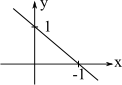
\includegraphics[scale=1.0]{capitulos/capitulo4/figuras/sol_sist_equa_m_equa_n_incog1.png}
 \caption{?}
 \label{fig:sol_sist_equa_m_equa_n_incog1}
\end{figure}

Por exemplo,

\[
 \left\{
  \begin{array}{rrrrrrrrrrr}
   -1 \, u & + & 2 \, v & + & 2 \, w & + & x & - & 2 \, y & = & 2\\
   3 \, u & - & 6 \, v & - & w & + & 5 \, x & - & 4 \,y & = & 1\\
   2 \, u & - & 4 \, v & - & 1.5 \, w & + & 2 \, x & - & y & = & -0.5
  \end{array}
 \right.
\]

\[
 \begin{array}{|rrrrrr|}
	\hline
	\textbf{u} & \textbf{v} & \textbf{w} & \textbf{x} & \textbf{y} & \textbf{l.d.}\\
	\hline \hline
	-1 & 2 & 2 & 1 & -2 & 2\\
	\hline
	3 & -6 & -1 & 5 & -4 & 1\\
	\hline
	2 & -4 & -1.5 & 2 & -1 & -0.5\\
	\hline
 \end{array}
\]

\begin{description}

\item[i)] Pivotação

\hspace*{2 cm}
$
 \left\{
  \begin{array}{rrrrrr|r}
   3 & -6 & -1 & 5 & -4 & 1 &\\
   -1 & 2 & 2 & 1 & -2 & 2 & L'_2 = L_2 + \frac{1}{3} \, L_1\\
   2 & -4 & -1.5 & 2 & -1 & -0.5 & L'_3 = L_3 - \frac{2}{3} \, L_1
  \end{array}
 \right.
$

\hspace*{2 cm}
$
 \left\{
  \begin{array}{lrlrrr|c}
   3^{\mbox{\tiny{(PIVÔ)}}} & -6 & -1 & 5 & -4 & 1 &\\
   0 & 0 & 5/3^{\mbox{\tiny{(PIVÔ)}}} & 8/3 & - 10/3 & - 7/3 &\\
   0 & 0 & - 5/6 & - 4/3 & 5/3 & - 7/6 & L'_3 = L_3 - \frac{1}{2} \, L_2
  \end{array}
 \right.
$

\hspace*{2 cm}
$
 \left\{
  \begin{array}{rrrrrr}
   3 & -6 & -1 & 5 & -4 & 1\\
   0 & 0 & 5/3 & 8/3 & - 10/3 & - 7/3\\
   0 & 0 & 0 & 0 & 0 & 0
  \end{array}
 \right.
$

\hspace*{2 cm}
$
 \left[
  \begin{array}{cc}
   3 & -1\\
   0 & 5/3
  \end{array}
 \right]
 \left[
  \begin{array}{c}
   u\\
   w
  \end{array}
 \right]
 =
 \left[
  \begin{array}{cccccc}
   u & = & 0.8 & + 2 \, v & -2.2 \, x & + 2 \,y\\
   w & = & 1.4 &          & -1.6 \, x & + 2 \,y
  \end{array}
 \right]
$

\end{description}

Exemplo 2: Gauss-Jordan

\[
 \begin{array}{|rrrrrr|}
	\hline
	\textbf{u} & \textbf{v} & \textbf{w} & \textbf{x} & \textbf{y} & \textbf{l.d.}\\
	\hline \hline
	2 & 3 & 1 & 4 & 1 & 6\\
	\hline
	2 & 3 & 1 & 1 & -1 & 1\\
	\hline
	4 & 6 & -1 & 1 & 2 & 5\\
	\hline
 \end{array}
\]

\begin{description}

\item[i)] Pivotação

\hspace*{2 cm}
$
 \left\{
  \begin{array}{rrrrrr|l}
   4 & 6 & -1 & 1 & 2 & 5 & (: 4)\\
   2 & 3 & 1 & 1 & -1 & 1 & L'_2 = L_2 - 2 \, L_1\\
   2 & 3 & 1 & 4 & 1 & 6 & L'_3 = L_3 - 2 \, L_1
  \end{array}
 \right.
$

\hspace*{2 cm}
$
 \left\{
  \begin{array}{rrrrrr|l}
   1 & 1.5 & -0.25 & 0.25 & 0.5 & 1.25 & L'_1 = L_1 + 0.25 \, L_2\\
   0 & 0 & 1.5 & 0.5 & -2 & -1.5 & (: 1.5)\\
   0 & 0 & 1.5 & 3.5 & 0 & 3.5 & L'_3 = L_3 - 1.5 \, L_2
  \end{array}
 \right.
$

\hspace*{2 cm}
$
 \left\{
  \begin{array}{rrrrrr|l}
   1 & 1.5 & 0 & 0.3333 & 0.1667 & 1 &\\
   0 & 0 & 1 & 0.3333 & -1.3333 & -1 &\\
   0 & 0 & 0 & 3 & 2 & 5 & (: 3)
  \end{array}
 \right.
$

\hspace*{2 cm}
$
 \left\{
  \begin{array}{rrrrrr|l}
   1 & 1.5 & 0 & 1/3 & 1/6 & 1 & L'_1 = L_1 - \frac{1}{3} \, L_3\\
   0 & 0 & 1 & 1/3 & -4/3 & -1 & L'_2 = L_2 - \frac{1}{3} \, L_3\\
   0 & 0 & 0 & 1 & 2/3 & 5/3 &
  \end{array}
 \right.
$

\end{description}

\textbf{OBS:} As variáveis básicas são aquelas cujos coeficientes são unitários e os únicos não nulos na coluna.

\hspace*{2 cm}
$
% \left\{
  \begin{array}{rrrr}
   u = & \displaystyle \frac{4}{9}    & - \, \displaystyle \frac{3}{2} \, v & + \displaystyle \frac{1}{18} \, y\\\\
   w = & - \, \displaystyle \frac{14}{9} &                 & + \displaystyle \frac{14}{9} \, y\\\\
   x = & \displaystyle \frac{5}{3}    &                 & + \displaystyle \frac{2}{3} \, y
  \end{array}
% \right.
$
